Este capítulo describe la gestión del proyecto: la metodología de desarrollo adoptada, las tecnologías y herramientas empleadas, la planificación temporal, los costes estimados, los riesgos identificados, la gestión de la configuración y las prácticas de aseguramiento de la calidad.

\section{Metodología de desarrollo}
\label{sec:metodologia}

El desarrollo del proyecto sigue un modelo incremental organizado en bloques de trabajo secuenciales. Cada bloque produce un entregable funcional que se integra con los anteriores: primero los motores de generación de oraciones, después la evaluación comparativa, a continuación la aplicación móvil y, en paralelo, la redacción de la memoria.

Al tratarse de un trabajo individual sin equipo de desarrollo, las metodologías ágiles basadas en equipos multidisciplinares (Scrum, Kanban) resultan artificiales: no hay \textit{daily standups} cuando el equipo es una sola persona, ni tiene sentido definir roles de \textit{product owner} y \textit{scrum master} cuando recaen en el mismo individuo.

El modelo incremental, en cambio, permite avanzar de forma ordenada sin la sobrecarga ceremonial de un \textit{framework} ágil, manteniendo la flexibilidad necesaria para incorporar cambios a medida que se obtienen resultados.

Las revisiones periódicas con las tutoras del TFG funcionan como puntos de control. Cada revisión evalúa el trabajo completado hasta la fecha, identifica problemas y reorienta las siguientes fases si es necesario. Se han planificado cuatro hitos de revisión a lo largo del proyecto:

\begin{enumerate}
    \item Revisión del prolegómeno de la memoria (enero de 2026).
    \item Revisión de la memoria sobre el desarrollo de los motores de generación de oraciones (marzo de 2026).
    \item Revisión de la memoria sobre el desarrollo de la aplicación móvil (abril de 2026).
    \item Revisión de la memoria final completa (mayo de 2026).
\end{enumerate}

\section{Herramientas de gestión y soporte}
\label{sec:tecnologias-herramientas}

Las tecnologías empleadas en cada una de las implementaciones se describen en los capítulos de desarrollo correspondientes. Para la gestión y el soporte del proyecto se utilizan cuatro herramientas. GitHub aloja los repositorios del código fuente, organizados de forma independiente por componente. Google Sheets se emplea como cronograma de seguimiento, donde se registran las tareas planificadas, sus fechas estimadas y su estado. Overleaf es el entorno de edición de la memoria en LaTeX, con sincronización automática contra un repositorio Git. Claude Code actúa como asistente de desarrollo con inteligencia artificial durante la implementación y la redacción.

\section{Planificación temporal}
\label{sec:planificacion}

El proyecto se desarrolla entre diciembre de 2025 y julio de 2026, con dos posibles convocatorias de defensa (junio y julio). La distribución de las tareas y los solapamientos entre los distintos bloques de trabajo se recogen en el diagrama de la Figura~\ref{fig:gantt}.

\begin{figure}[ht]
    \centering
    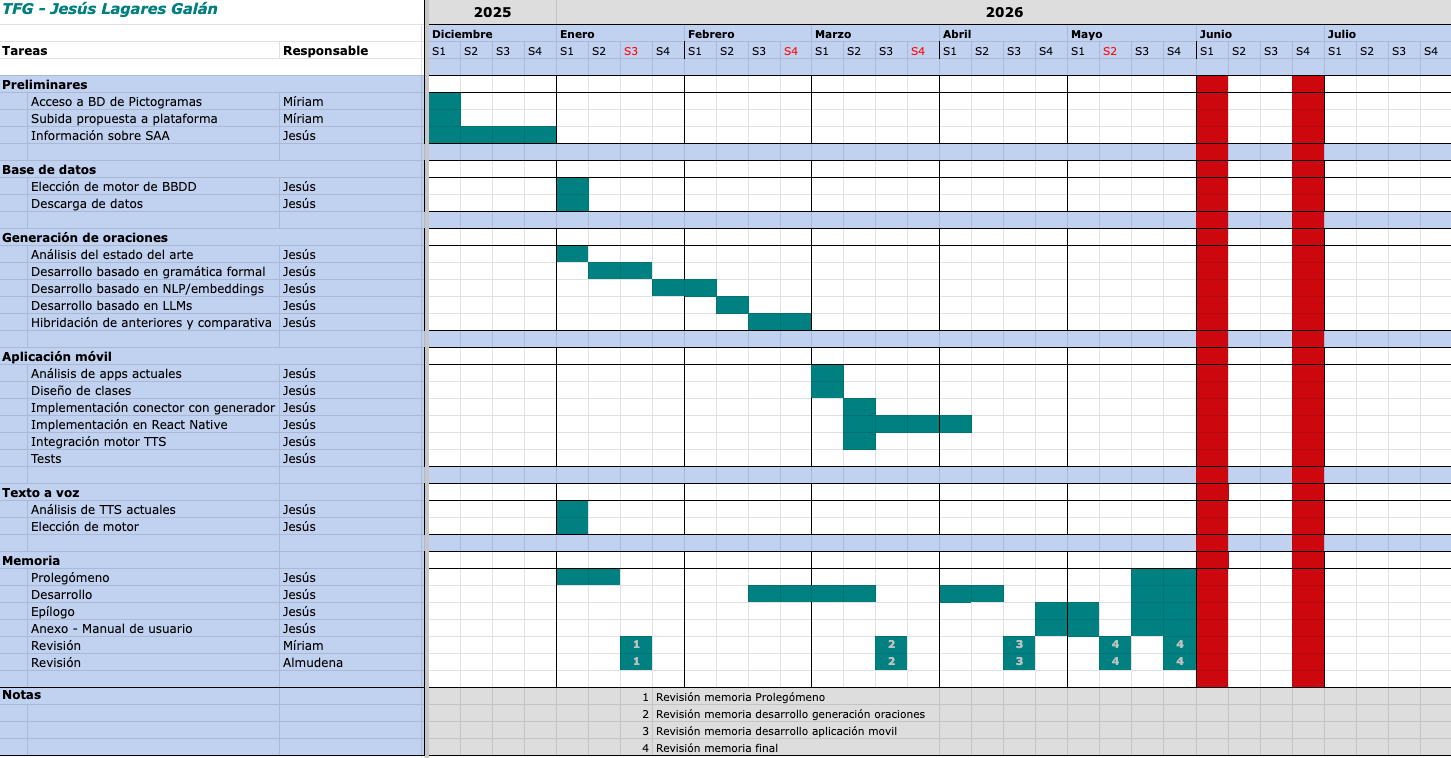
\includegraphics[width=\textwidth]{figures/gantt.png}
    \caption{Diagrama de Gantt con la planificación temporal del proyecto. Las franjas rojas marcan las dos convocatorias de defensa (junio y julio de 2026) y los números sobre las filas inferiores identifican los cuatro hitos de revisión de la memoria.}
    \label{fig:gantt}
\end{figure}

\section{Estimación de costes}
\label{sec:costes}

Al tratarse de un Trabajo de Fin de Grado, la estimación de costes se limita a los servicios externos que el sistema consume en ejecución. El trabajo del alumno, la supervisión de las tutoras y el equipo de desarrollo no se computan como gasto al formar parte de la dedicación académica propia del TFG, y el resto de herramientas empleadas son gratuitas o de código abierto.

La API de OpenAI~\cite{openai2024pricing} se utiliza en el motor de modelos de lenguaje y en las hibridaciones que lo incorporan. A precios de abril de 2026, GPT-4o factura \$2.50 por millón de tokens de entrada y \$10.00 por millón de salida, mientras que GPT-4o-mini se queda en \$0.15 y \$0.60 respectivamente; el desglose del coste por consulta aparece en la sección~\ref{ch:modelos-lenguaje}.

La API de ElevenLabs~\cite{elevenlabs2026pricing}, prevista para la síntesis de voz neuronal en la aplicación móvil, factura por caracteres: \$0.06 por cada 1.000 caracteres con los modelos \textit{Flash} y \textit{Turbo}, y \$0.12 con los modelos \textit{Multilingual v2} y \textit{v3}.

\section{Gestión de riesgos}
\label{sec:riesgos}

El desarrollo del proyecto está condicionado por cinco riesgos relevantes.

El tamaño del modelo de FastText utilizado por el enfoque de embeddings condiciona el despliegue. El modelo preentrenado sobre el corpus \textit{Spanish Billion Words} ocupa 6,7 GB en disco, lo que descarta funciones \textit{serverless} y servicios con restricciones de memoria. La mitigación consiste en desplegar el servidor mediante contenedores Docker con disco suficiente, lo que restringe la infraestructura pero no impide el funcionamiento.

La dependencia de la API de OpenAI afecta al motor de modelos de lenguaje y a las dos hibridaciones que lo incorporan: sin acceso a Internet, la mitad de las técnicas deja de operar. El servidor implementa \textit{fallback} automático a la gramática formal y a la gramática enriquecida con embeddings, que funcionan en local y permiten seguir dando servicio.

El vocabulario cerrado del sistema, limitado a 232 pictogramas de ARASAAC, deja fuera cualquier concepto no representado. La mitigación se abordó en la fase de selección, priorizando los conceptos más frecuentes en la comunicación cotidiana de usuarios de CAA y cubriendo nueve categorías semánticas.

La evaluación comparativa podría producir resultados inconcluyentes y comprometer las conclusiones del proyecto. Para minimizar este riesgo se combinan métricas automáticas (BLEU, ROUGE, BERTScore, perplejidad) con evaluación humana mediante encuestas, y se aplica el test de Wilcoxon~\cite{wilcoxon1945individual} con corrección para comparaciones múltiples, que permite discriminar qué diferencias entre técnicas son estadísticamente significativas.

La compatibilidad multiplataforma de la aplicación móvil introduce diferencias de comportamiento entre iOS y Android en renderizado, animaciones y acceso a APIs nativas. Se mitiga apoyándose en Expo como capa de abstracción, que unifica las APIs para la mayoría de funcionalidades que la aplicación necesita.

\section{Aseguramiento de la calidad}
\label{sec:calidad}

Las prácticas de aseguramiento de la calidad del proyecto abarcan cuatro niveles: verificación unitaria de los motores, evaluación comparativa automatizada, evaluación humana y verificación del servidor y la aplicación.

Los motores de generación de oraciones incorporan tests unitarios que verifican el comportamiento de cada componente de forma aislada: concordancias de género y número, inserción de determinantes y preposiciones, conjugación verbal, restricciones de selección semánticas e inferencia de elementos faltantes, entre otros. Estos tests permiten detectar regresiones cuando se modifican las reglas o los parámetros de los motores.

La evaluación comparativa automatizada constituye el segundo nivel de verificación. Un \textit{pipeline} ejecuta los seis motores sobre un conjunto de 130 casos de prueba y calcula para cada uno las métricas BLEU~\cite{papineni2002bleu}, ROUGE~\cite{lin2004rouge}, BERTScore~\cite{zhang2020bertscore} y perplejidad, entre otras. Los resultados se someten a tests de significancia estadística (Wilcoxon~\cite{wilcoxon1945individual} con corrección de Holm) para determinar si las diferencias entre técnicas son estadísticamente significativas. Los detalles de este proceso se describen en la sección~\ref{ch:evaluacion-comparativa}.

La evaluación humana complementa las métricas automáticas con la percepción de personas reales. Se diseñaron encuestas con escalas Likert de 7 puntos para medir la naturalidad percibida de las oraciones generadas y su proximidad a una referencia \textit{gold standard}. Este proceso, junto con sus resultados, se detalla en la sección~\ref{ch:evaluacion-comparativa}.

En la aplicación móvil, el uso de TypeScript como lenguaje de desarrollo proporciona tipado estático que detecta inconsistencias de tipos en tiempo de compilación. El servidor REST implementa \textit{endpoints} de salud (\textit{liveness} y \textit{readiness}) que permiten verificar automáticamente si el servicio está operativo y si los motores de generación están cargados y listos para procesar peticiones.
